%=============================================================================
%  Section 3 -- Two cost laws
%  Every number is a macro from macros.tex (authority: paper/NUMBERS.md).
%  Numbers still lacking a macro are marked \needsnum{proposed-macro-name}.
%=============================================================================
\section{Two Cost Laws}
\label{sec:cost-laws}

The first question a serving study must answer is what a request costs. For an
autoregressive model the answer is folklore: cost is proportional to the number
of tokens emitted. For a diffusion language model it is not folklore, and the
difference is the origin of every result in this paper. This section fits both
laws on the same hardware, the same runtime and the same data, validates them by
extrapolation, and then shows that the diffusion law's invariance to output
length holds not only in cost but --- unexpectedly --- in \emph{quality}.

\subsection{Setup}
\label{sec:cost-laws:setup}

All measurements in this section come from a single machine and a single
runtime: one NVIDIA A100 80\,GB PCIe, vLLM 0.25.1, BF16 weights, serial serving
(\texttt{-{}-max-num-seqs 1}), so that every reported latency is a
single-request service time uncontaminated by scheduling. The workload is
structured extraction over BGL system logs (LOGHUB, temporal split, test
partition); the task emits a 12-field JSON record per event. We sweep a forced
output length $L$ by setting \texttt{min\_tokens} $=$ \texttt{max\_tokens} $=L$
and measure $n=300$ requests per cell. The two models are \modelDG{} (a block
diffusion model; mixture-of-experts, 26\,B total parameters) and \modelARthree{}
(dense autoregressive). Sizes are not matched; we return to that in the threats
section. The cost laws below are per-model measurements and do not depend on the
comparison being size-matched.

\subsection{The two laws}
\label{sec:cost-laws:laws}

Least-squares fits over $L \in \{32,64,128,256,512,1024,2048\}$ give
%
\begin{align}
  \costLawAR \quad [\si{\milli\second}],
  \label{eq:law-ar}\\[2pt]
  \costLawDG \quad [\si{\milli\second}].
  \label{eq:law-dg}
\end{align}
%
Equation~\eqref{eq:law-ar} is the expected linear law: residual
$\sigma = \arResidSigma$\,ms across the whole sweep, with no visible curvature
out to $L=2048$. Equation~\eqref{eq:law-dg} is not linear at all. It is a
\emph{step} function. The diffusion model denoises a fixed canvas of
\dgCanvas{} tokens; every output length that fits inside one canvas costs the
same \dgBase{}\,ms, and only crossing a canvas boundary adds cost, at
\dgStep{}\,ms per additional block. Within a canvas, generating one token and
generating \dgCanvas{} tokens are the same operation performed the same number
of times.

\open{The AR fit is not yet internally consistent across our own artifacts:
\texttt{appD\_analysis.json} gives intercept \arIntercept{}, slope \arSlope{},
$\sigma=\arResidSigma$\,ms, while \texttt{appD\_report.md} reports a different
intercept and $\sigma$ for the same data. We use the JSON throughout. The fit
must be re-run from raw per-cell data and reconciled before submission.}

\subsection{Derived quantities}
\label{sec:cost-laws:derived}

Four numbers follow from Eqs.~\eqref{eq:law-ar}--\eqref{eq:law-dg} and carry the
rest of the paper.

\begin{description}
  \item[Marginal cost.] Autoregressive decoding costs \arSlope{}\,ms per
    generated token. Diffusion's \emph{amortised} marginal cost is
    $\dgStep/\dgCanvas = \dgMarginal$\,ms per token --- and even that overstates
    it, since the true marginal cost of a token inside an already-open canvas is
    zero.
  \item[Asymptotic ratio.] As $L \to \infty$ the ratio of the two laws tends to
    $\arSlope/\dgMarginal = \asymptoticRatio\times$. The diffusion advantage
    does not grow without bound; it saturates.
  \item[Length crossover.] The laws cross at $L \approx \lengthCrossover$
    tokens. Below it the autoregressive model is cheaper --- it pays only for
    what it emits, while the diffusion model pays for a whole canvas regardless.
  \item[Natural output length.] The task's own 12-field record is
    $\sim\naturalOutput$ tokens.
\end{description}

\noindent
The last two numbers should be read together, and stated explicitly because they
explain results reported before this paper. The task's natural output,
$\sim\naturalOutput$ tokens, sits \emph{just above} the crossover at
$\lengthCrossover$ tokens --- above it, but by well under a factor of three, and
still comfortably inside a single \dgCanvas{}-token canvas. Every single-request
latency comparison on this task is therefore taken from a point that is barely
inside the diffusion model's favourable regime. A task with slightly shorter
records would have reversed the sign of the comparison; a task with much longer
records would have inflated it toward \asymptoticRatio$\times$. The
single-request latency advantage reported in earlier work on this workload is
not a property of diffusion decoding in general. It is a property of where this
particular task's output length falls relative to
$L \approx \lengthCrossover$.

\subsection{Validating the laws by extrapolation}
\label{sec:cost-laws:validation}

Both laws were fitted on $L \le 512$ and then used to predict two held-out
lengths. Equation~\eqref{eq:law-dg} predicts \dgPredKiloOneK{}\,ms at $L=1024$
(measured \dgMeasKiloOneK{}\,ms, $+\dgErrKiloOneK$\%) and \dgPredTwoK{}\,ms at
$L=2048$ (measured \dgMeasTwoK{}\,ms, $+\dgErrTwoK$\%). Both are within 15\%,
and both err in the same direction, consistent with a small per-canvas overhead
the two-parameter step model does not capture. The autoregressive slope
\arSlope{}\,ms/token remains linear to $L=2048$ with no fitted correction. The
functional forms --- linear versus stepwise --- are therefore not artefacts of
the fitted range.

\subsection{Measured latency across the sweep}
\label{sec:cost-laws:table}

Table~\ref{tab:latency-by-l} gives the underlying measurements.

\begin{table}[t]
  \centering
  \caption{Single-request latency (p50) by forced output length $L$.
    A100 80\,GB PCIe, vLLM 0.25.1, BF16, \texttt{-{}-max-num-seqs 1},
    $n=300$ per cell. The autoregressive model wins below the crossover at
    $L \approx \lengthCrossover$; the diffusion model is flat inside each
    \dgCanvas{}-token canvas.}
  \label{tab:latency-by-l}
  \begin{tabular}{rrrr}
    \toprule
    $L$ (tokens) & $T_{\mathrm{AR}}$ p50 (ms) & $T_{\mathrm{DG}}$ p50 (ms) & AR/DG \\
    \midrule
    32   & \needsnum{arPFiftyThirtyTwo}  & \needsnum{dgPFiftyThirtyTwo}  & \needsnum{ratioThirtyTwo} \\
    64   & \needsnum{arPFiftySixtyFour}  & \needsnum{dgPFiftySixtyFour}  & \needsnum{ratioSixtyFour} \\
    128  & \needsnum{arPFiftyOneTwoEight}& \needsnum{dgPFiftyOneTwoEight}& \needsnum{ratioOneTwoEight} \\
    256  & \needsnum{arPFiftyTwoFiveSix} & \needsnum{dgPFiftyTwoFiveSix} & \needsnum{ratioTwoFiveSix} \\
    512  & \needsnum{arPFiftyFiveTwelve} & \needsnum{dgPFiftyFiveTwelve} & \needsnum{ratioFiveTwelve} \\
    1024 & \needsnum{arPFiftyKiloOneK}   & \dgMeasKiloOneK               & \needsnum{ratioKiloOneK} \\
    2048 & \needsnum{arPFiftyTwoK}       & \dgMeasTwoK                   & \needsnum{ratioTwoK} \\
    \bottomrule
  \end{tabular}
\end{table}

\begin{figure}[t]
  \centering
  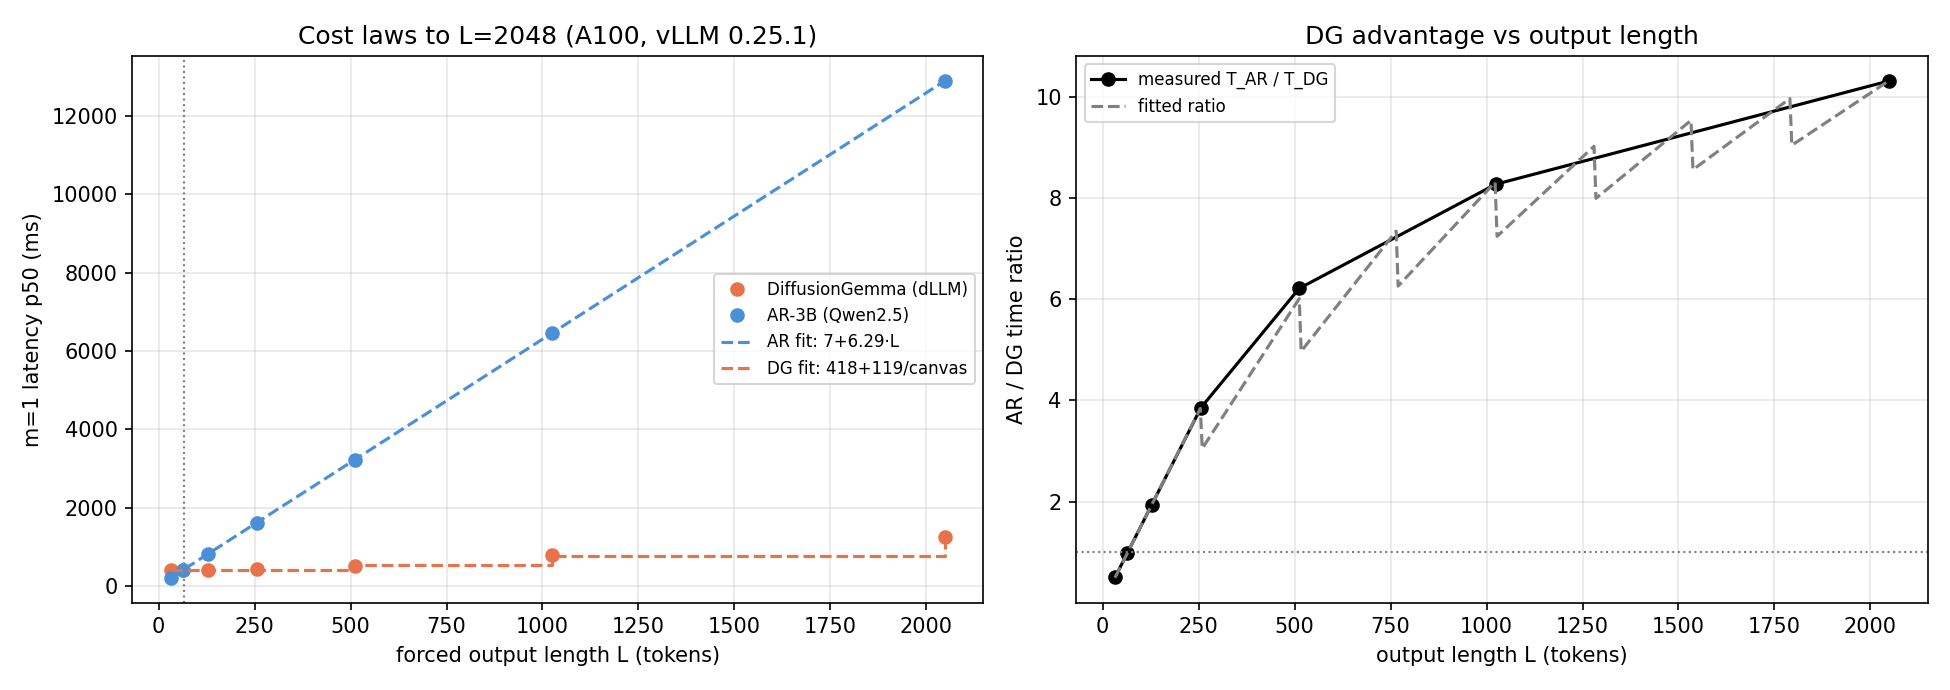
\includegraphics[width=0.92\textwidth]{../results/appD_costlaws.png}
  \caption{Measured cost curves and their ratio. The autoregressive curve is a
    line through the origin; the diffusion curve is a staircase with treads of
    width \dgCanvas{} tokens. \todo{chart will be regenerated for print --
      match fonts, drop the interactive legend, mark the crossover at
      $L=\lengthCrossover$ and the natural output at $L=\naturalOutput$.}}
  \label{fig:cost-laws}
\end{figure}

\subsection{Quality is also length-invariant}
\label{sec:cost-laws:quality}

The cost laws are the expected part of the result. The unexpected part is that
the same invariance appears in extraction quality. We re-scored every cell of
the sweep --- the identical runs, $n=300$ each, with output length forced to $L$
--- on field-level F1 and on schema validity (the fraction of outputs that parse
as a complete record). Table~\ref{tab:quality-by-l} gives the result. It has
three regimes, and they do not point the same way.

\begin{table}[t]
  \centering
  \caption{Extraction quality by forced output length $L$. Same runs as
    Table~\ref{tab:latency-by-l}; $n=300$ per cell. ``valid'' is the percentage
    of outputs that parse as a complete schema record. Three regimes:
    truncation ($L \le 128$), matched ($L=256$, near the natural
    $\sim\naturalOutput$ tokens), over-generation ($L \ge 512$).}
  \label{tab:quality-by-l}
  \begin{tabular}{rrrrrl}
    \toprule
    $L$ & DG F1 & DG valid (\%) & AR F1 & AR valid (\%) & regime \\
    \midrule
    32   & \needsnum{dgFOneThirtyTwo} & \needsnum{dgValidThirtyTwo} & \needsnum{arFOneThirtyTwo} & \needsnum{arValidThirtyTwo} & truncation \\
    64   & \needsnum{dgFOneSixtyFour} & \needsnum{dgValidSixtyFour} & \needsnum{arFOneSixtyFour} & \needsnum{arValidSixtyFour} & truncation \\
    128  & \dgFOneOneTwoEight & \dgValidOneTwoEight & \textbf{\arFOneOneTwoEight} & \arValidOneTwoEight & truncation \\
    256  & \dgFOneTwoFiveSix  & \needsnum{dgValidTwoFiveSix} & \textbf{\arFOneTwoFiveSix} & \needsnum{arValidTwoFiveSix} & matched \\
    512  & \textbf{\dgFOneFiveTwelve} & \needsnum{dgValidFiveTwelve} & \arFOneFiveTwelve & \needsnum{arValidFiveTwelve} & over-gen. \\
    1024 & \textbf{\dgFOneKiloOneK}   & \needsnum{dgValidKiloOneK}  & \arFOneKiloOneK   & \needsnum{arValidKiloOneK}  & over-gen. \\
    2048 & \textbf{\dgFOneTwoK}       & \needsnum{dgValidTwoK}      & \arFOneTwoK       & \needsnum{arValidTwoK}      & over-gen. \\
    \bottomrule
  \end{tabular}
\end{table}

\paragraph{(a) Truncation ($L \le 128$): an autoregressive advantage.}
When the budget is below what the record needs, both models fail --- but they
fail differently, and the difference favours autoregression. At $L=128$ the
autoregressive model scores \arFOneOneTwoEight{} F1 with \arValidOneTwoEight\%
of outputs parseable; the diffusion model scores \dgFOneOneTwoEight{} with
\dgValidOneTwoEight\%. The mechanism is decoding order. Left-to-right decoding
truncated at $L$ emits a valid \emph{prefix} of the record: the first several
fields are complete and correct, and a lenient parser recovers them. Joint
denoising truncated mid-canvas emits nothing parseable --- the canvas has not
converged anywhere, so no field is finished. Autoregression degrades gracefully
under a length budget; block diffusion degrades catastrophically. We report this
as an autoregressive advantage because it is one, and it is the exact mirror
image of regime~(c).

\paragraph{(b) Matched ($L=256$).}
At the first length that comfortably contains the natural $\sim\naturalOutput$-token
record, the autoregressive model is modestly ahead: \arFOneTwoFiveSix{} versus
\dgFOneTwoFiveSix{}. Both are near-fully valid. This is the honest
apples-to-apples quality comparison for this task, and diffusion loses it
slightly.

\paragraph{(c) Over-generation ($L \ge 512$): the invariance result.}
Above the natural length the two models separate, and they separate in the
direction the cost laws predict but for reasons the cost laws do not cover. The
diffusion model is \emph{flat}: \dgFOneFiveTwelve{}, \dgFOneKiloOneK{},
\dgFOneTwoK{} at $L=512$, $1024$, $2048$, with 100\% schema validity throughout.
Quadrupling the token budget changes its F1 in the third decimal place. The
autoregressive model decays \emph{monotonically} over the same range:
\arFOneFiveTwelve{}, \arFOneKiloOneK{}, \arFOneTwoK{}. Taken with the matched
cell, that is a four-point monotone decline at $n=300$ per cell, from
\arFOneTwoFiveSix{} at $L=256$ to \arFOneTwoK{} at $L=2048$ --- a loss of
roughly a third of the model's F1, purchased with nothing but a larger
\texttt{max\_tokens}.

\paragraph{What over-generation actually damages.}
The per-field breakdown at $L=512$ locates the damage precisely, and it lands
where it should not. The \texttt{host} field is a verbatim copy from the input:
the correct behaviour is transcription, not inference. The autoregressive model
scores \arHostFiveTwelve{} on it; the diffusion model scores
\dgHostFiveTwelve{}. Overall anomaly-F1 tells the same story more sharply ---
\arAnomalyFOneFiveTwelve{} versus \dgAnomalyFOneFiveTwelve{}
(Table~\ref{tab:per-field-512}). Forced to keep emitting past the end of the
record, the autoregressive model does not simply idle: it continues generating,
and what it generates conditions and corrupts fields it has already been asked
to copy. Over-generation is not merely wasted time. It degrades extraction that
ought to be immune to output length altogether.

\begin{table}[t]
  \centering
  \caption{Per-field F1 at $L=512$ ($n=300$). The autoregressive model's largest
    losses are on fields that require copying, not inference.}
  \label{tab:per-field-512}
  \begin{tabular}{lrr}
    \toprule
    Field & AR ($L=512$) & DG ($L=512$) \\
    \midrule
    \texttt{host}            & \arHostFiveTwelve & \dgHostFiveTwelve \\
    \texttt{component}       & \needsnum{arComponentFiveTwelve} & \needsnum{dgComponentFiveTwelve} \\
    \texttt{severity}        & \needsnum{arSeverityFiveTwelve}  & \needsnum{dgSeverityFiveTwelve} \\
    \texttt{timestamp\_norm} & \needsnum{arTimestampFiveTwelve} & \needsnum{dgTimestampFiveTwelve} \\
    \texttt{is\_anomaly}     & \needsnum{arIsAnomalyFiveTwelve} & \needsnum{dgIsAnomalyFiveTwelve} \\
    \midrule
    anomaly-F1 (overall)     & \arAnomalyFOneFiveTwelve & \dgAnomalyFOneFiveTwelve \\
    \bottomrule
  \end{tabular}
\end{table}

\begin{figure}[t]
  \centering
  % \includegraphics[width=0.92\textwidth]{../results/quality_vs_length.png}
  \todo{FIGURE TO BE GENERATED -- \texttt{results/quality\_vs\_length.png} does
    not yet exist. Required: field-F1 versus forced output length $L$ for both
    models on one axis, with the three regimes shaded (truncation $L\le128$,
    matched $L=256$, over-generation $L\ge512$), a marker at the natural output
    $L=\naturalOutput$, and schema validity on a secondary axis. Data:
    \texttt{results/p2\_\{dg,ar3b\}\_L\{32,64,128,256,512\}.json} and
    \texttt{results/appD\_\{dg,ar3b\}\_L\{1024,2048\}.json}.}
  \caption{Quality versus forced output length. The diffusion curve is flat
    above the natural output length; the autoregressive curve peaks near it and
    declines monotonically thereafter, while being the only one of the two that
    survives truncation below it.}
  \label{fig:quality-vs-l}
\end{figure}

\subsection{The claim, and the claim we do not make}
\label{sec:cost-laws:claim}

Stated precisely: \emph{a block diffusion model's invariance to output length
holds in both cost and quality}. Equation~\eqref{eq:law-dg} gives the cost half
--- flat within a canvas, stepwise across canvases. Regime~(c) gives the quality
half --- flat F1 and 100\% validity from $L=512$ to $L=2048$. The
autoregressive model has neither: its cost is linear in tokens emitted
(Eq.~\eqref{eq:law-ar}) and its quality declines monotonically in tokens
emitted. Where the output length is not known in advance, or is set generously
for safety, that is a real operational property and not a benchmark artefact.

We do not claim that diffusion is \emph{more robust} in general. It is strictly
worse in the truncation regime --- \dgFOneOneTwoEight{} against
\arFOneOneTwoEight{} at $L=128$, and \dgValidOneTwoEight\% validity against
\arValidOneTwoEight\%, a gap far larger than any advantage it holds at
$L\ge512$. It is also slightly behind at the matched length. The invariance is
one-sided: it protects against over-provisioning the output budget, and it
offers no protection at all against under-provisioning it. A system that can
bound its output length tightly should prefer autoregression on this evidence;
a system that cannot should not assume that an over-generous budget is free,
because for the autoregressive model it is not.
